\documentclass[14pt]{beamer}
\usepackage{luatexja-fontspec}
\newjfontface{\nonproportional}{BIZ UDMincho}[YokoFeatures={JFM=ujis}]
\setmainjfont[Ligatures={Common,TeX},
  ItalicFont={BIZ UDPMincho},
  ItalicFeatures={FakeSlant=0.27},
  SlantedFont={BIZ UDPMincho},
  SlantedFeatures={FakeSlant=0.18},
  BoldFont={BIZ UDPGothic Bold},
  BoldSlantedFont={BIZ UDPGothic Bold},
  BoldSlantedFeatures={FakeSlant=0.18},
  BoldItalicFont={BIZ UDPGothic Bold},
  BoldItalicFeatures={FakeSlant=0.27},
  YokoFeatures={JFM=prop}]{BIZ UDPMincho}
%\newjfontface{\nonproportional}{BIZ UDGothic}[YokoFeatures={JFM=ujis}]
\setsansjfont[Ligatures={Common,TeX},
  ItalicFont={BIZ UDPGothic},
  ItalicFeatures={FakeSlant=0.23},
  SlantedFont={BIZ UDPGothic},
  SlantedFeatures={FakeSlant=0.23},
  BoldFont={BIZ UDPGothic Bold},
  BoldSlantedFont={BIZ UDPGothic Bold},
  BoldSlantedFeatures={FakeSlant=0.23},
  BoldItalicFont={BIZ UDPGothic Bold},
  BoldItalicFeatures={FakeSlant=0.23},
  YokoFeatures={JFM=prop}]{BIZ UDPGothic}
\usepackage{beamerthemesplit}
\usepackage{caption}
\captionsetup[figure]{labelformat=empty,labelsep=none}
\usepackage{svg}
\usepackage[]{graphicx}
\graphicspath{
  {./images/}
}
\svgsetup{
  inkscapelatex=false
}

\usepackage{listings,jvlisting}
\lstset{
  language=C++,
  basicstyle=\ttfamily\footnotesize,
  % keywordstyle=\bfseries\color{green},
  showstringspaces=false,
  frame={tb},
  %numbers=left,
  xrightmargin=0\zw,
  xleftmargin=0\zw,
  % columns=[l]{fullflexible},
  columns=fixed,
  basewidth=0.5em,
  numberstyle = \footnotesize,
  frame = tbrl,
  captionpos = b,
  moredelim=[is][\color{green}\bfseries]{<\#green\#}{\#>},
  moredelim=[is][\color{blue}\bfseries]{<\#blue\#}{\#>},
  moredelim=[is][\color{red}\bfseries]{<\#red\#}{\#>},
  moredelim=[is][\color{yellow}\bfseries]{<\#yellow\#}{\#>},
  moredelim=[is][\color{magenta}\bfseries]{<\#magenta\#}{\#>},
}

% 余白を広げる
\setbeamersize{text margin left=15pt, text margin right=15pt}
\setbeamertemplate{footline}[frame number]
\title{子どもIT未来塾 第6回}
\author{奥山 祐市}

\begin{document}

\frame{
   \begin{center}
    \huge{子どもIT未来塾}\\

    \vspace{48pt}
	   \Large{第6回}\\
	   {\huge\bf 音声合成と音声認識}\\
    \vspace{24pt}
    \large{奥山 祐市}
    \vspace{10pt}
    \large{\the\year 年 8月20日}
  \end{center}
}


\begin{frame}
	\frametitle{今日やること}
  \begin{enumerate}
    \item 音声合成
    \begin{enumerate}
      \item 音声合成とは
      \item Open JTalkとは
    \end{enumerate}
    \item 音声認識
    \begin{enumerate}
      \item 音声認識とは
      \item Juliusとは
    \end{enumerate}
  \end{enumerate}
\end{frame}

\begin{frame}
  \frametitle{音声合成}
  人間の音声を人工的に作りだすこと
  \begin{figure}
    \centering
    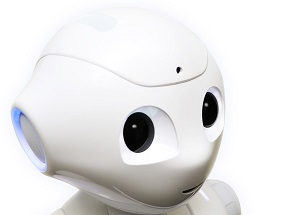
\includegraphics[width=0.5\textwidth]{chap06/text06-img001.jpg}
    \caption{Pepper (softbank)}
  \end{figure}
\end{frame}

\begin{frame}
  \frametitle{Open JTalk}
  \begin{itemize}
    \item 音声合成のためのソフトウェア
    \item 文字(テキスト)を読み上げる
  \end{itemize}
  \centering
  \includesvg[width=0.8\textwidth]{chap06/text06-img011.svg}
\end{frame}

\begin{frame}
  \frametitle{音声認識}
  \begin{itemize}
    \item 人間の声をコンピュータに認識させること
    \item 話し言葉から文字列への変換
    \item 音声の特徴を捉える
  \end{itemize}
  \note{画像を挿入}
\end{frame}

\begin{frame}
  \frametitle{Julius}
  \begin{itemize}
    \item 音声認識のためのソフトウェア
    \item 音声を聞き取って文字に変換する
  \end{itemize}
  \centering
  \includesvg[width=0.8\textwidth]{chap06/Julius.svg}
\end{frame}

\begin{frame}
  \frametitle{問題を解こう}
  \begin{itemize}
    \item 教科書2ページ 問題6-1
    \item 教科書2ページ 問題6-2
  \end{itemize}
\end{frame}

\begin{frame}
  \centering
  準備
\end{frame}

\begin{frame}
  \frametitle{ヘッドフォンをつけよう}
  \centering
  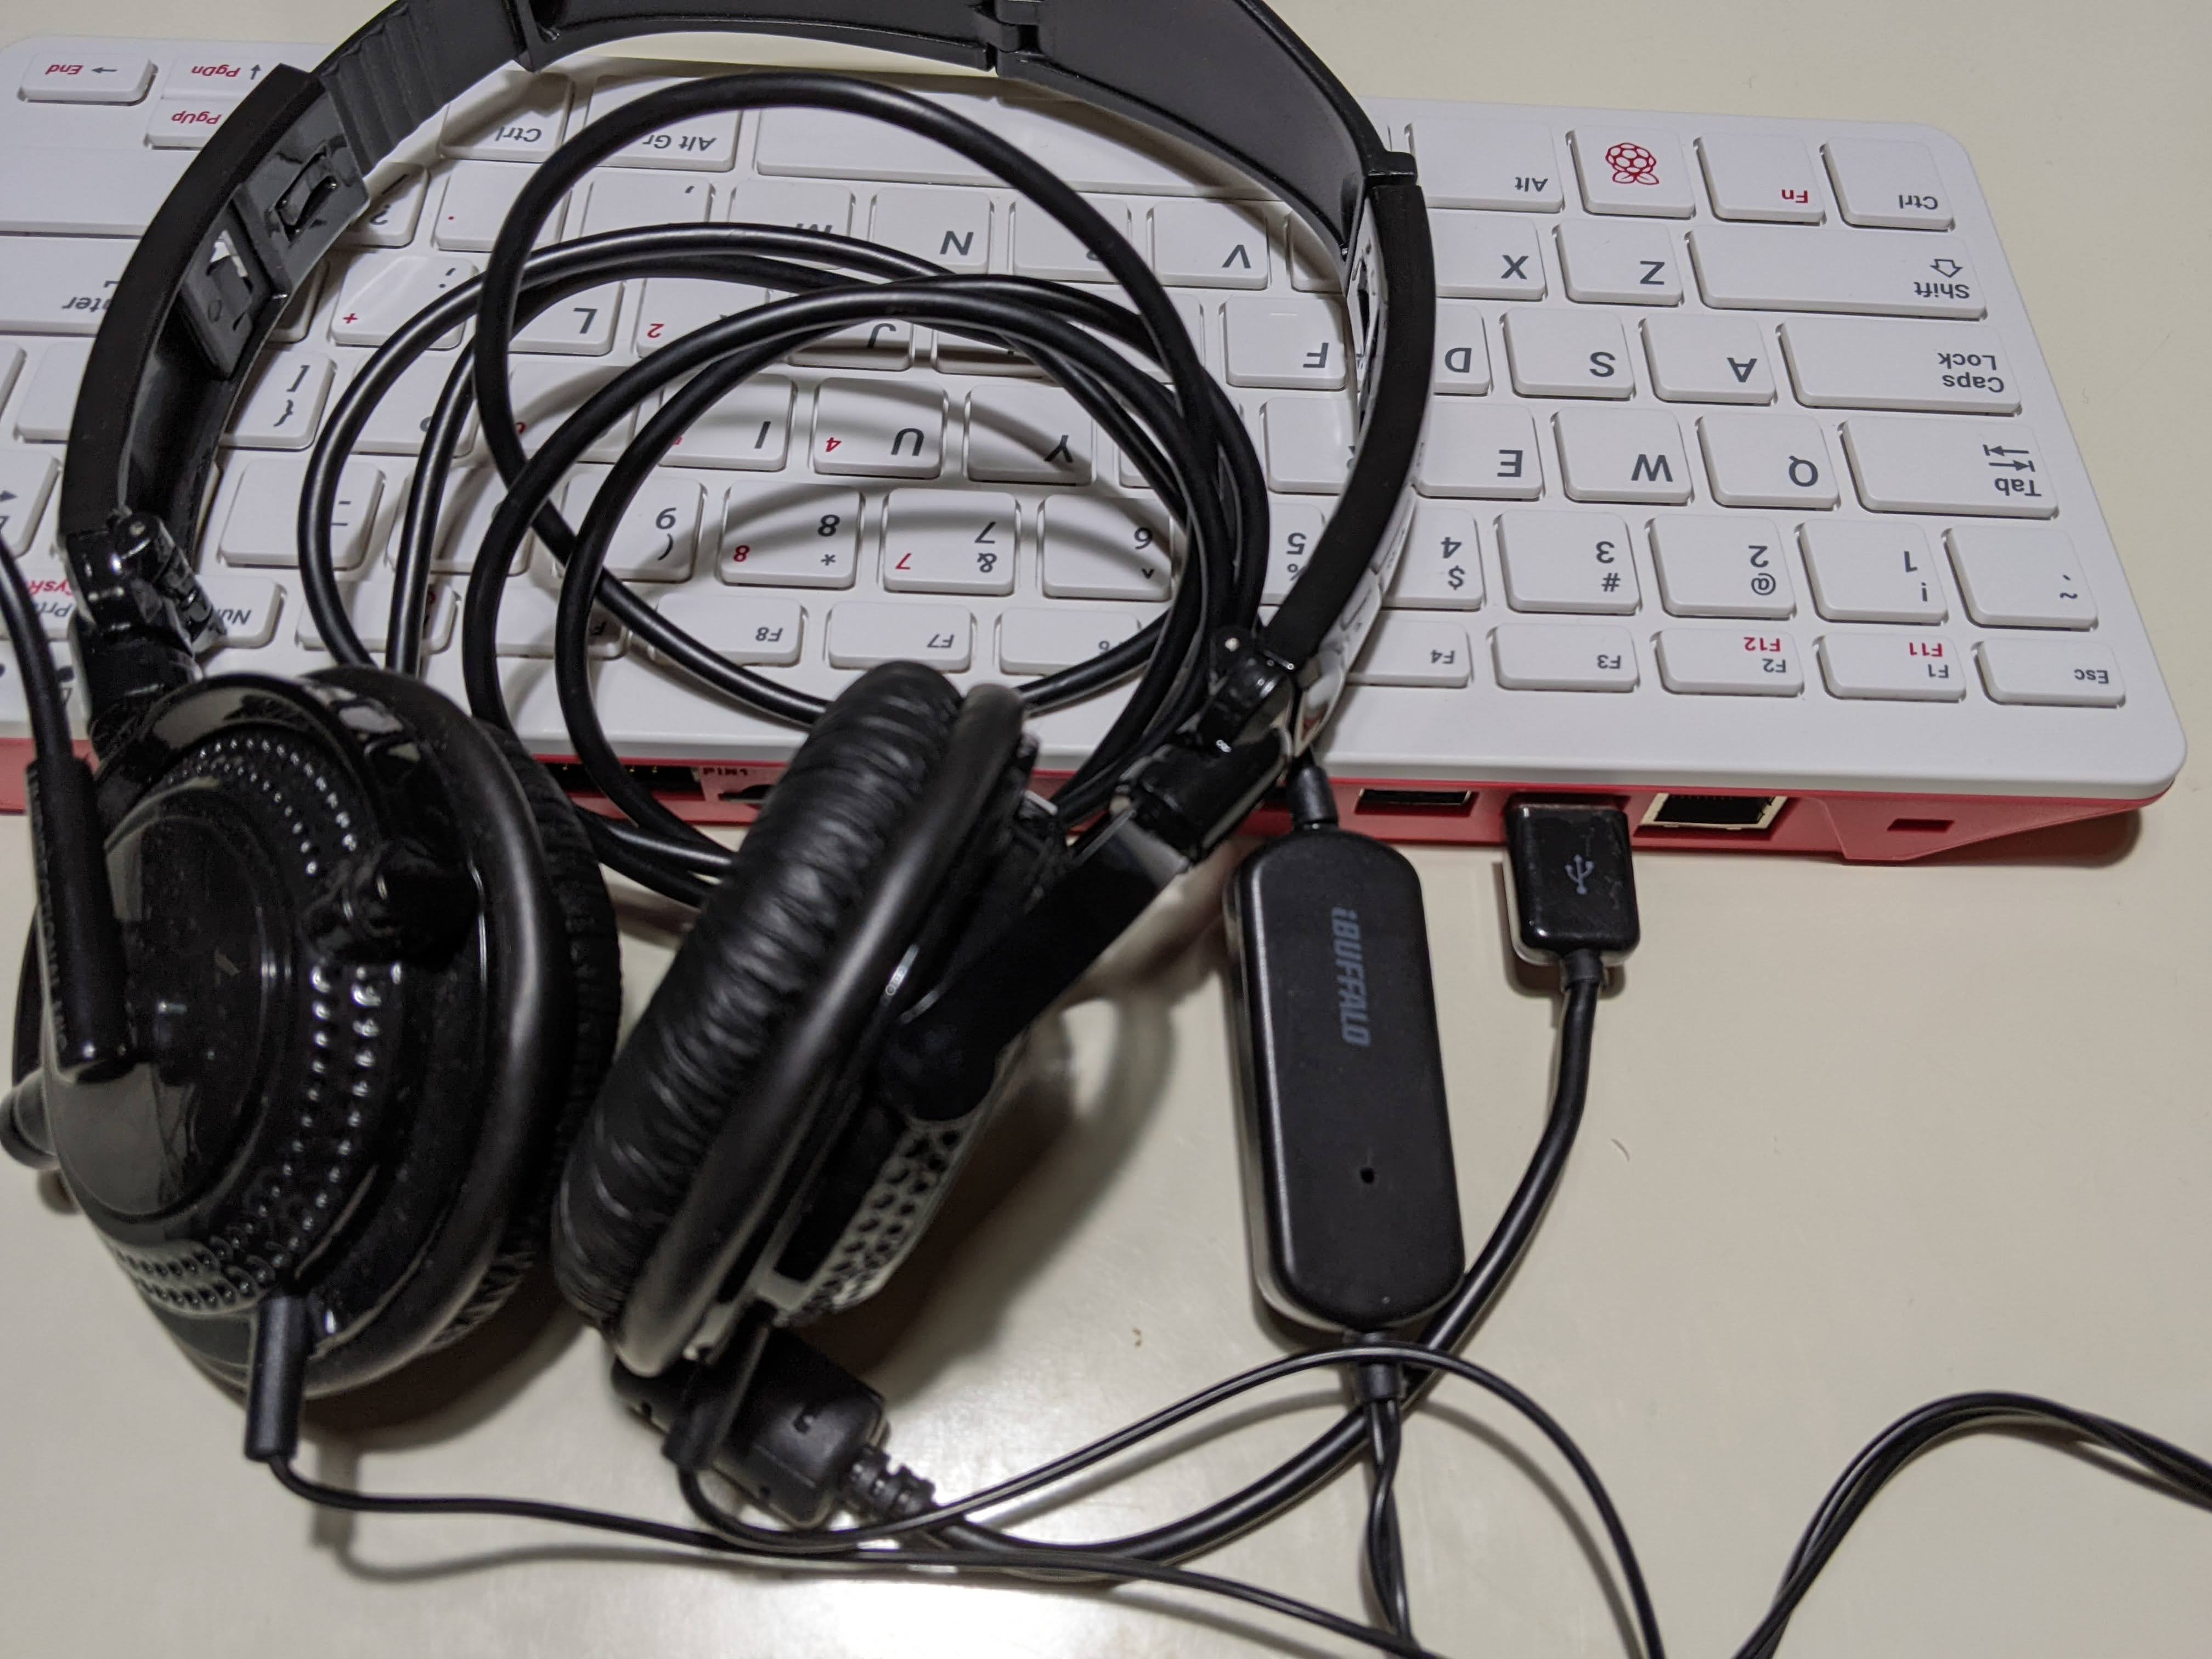
\includegraphics[width=0.8\textwidth]{how_to_connect_headset.jpg}
\end{frame}

\begin{frame}
  \frametitle{マイクミュートについて}
  \begin{itemize}
    \item ヘッドセットのコントローラに赤いランプが点いていると「マイクミュート」
    \item マイクを使うときはマイクミュートを解除しておこう
  \end{itemize}
  \centering
  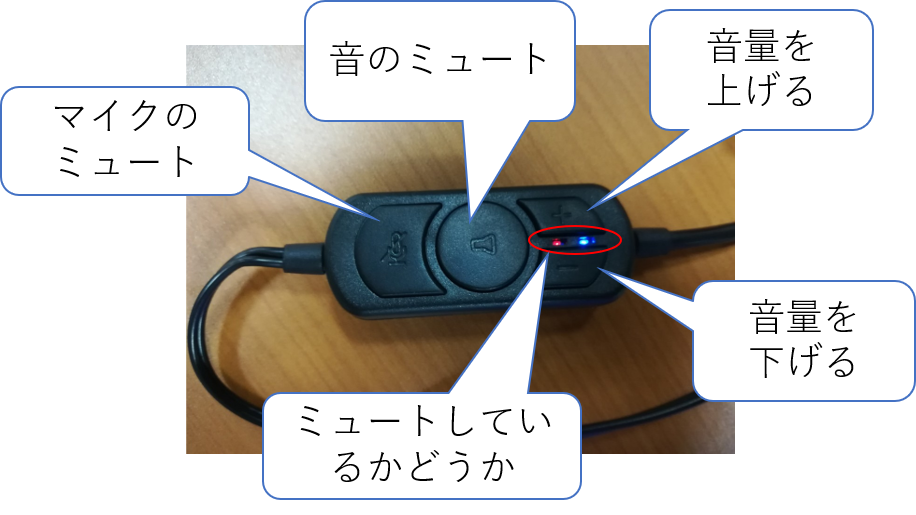
\includegraphics[width=0.8\textwidth]{chap06/text06-img004.png}
\end{frame}

\begin{frame}
  \frametitle{マイク音量の設定}

  \begin{figure}
    \centering
    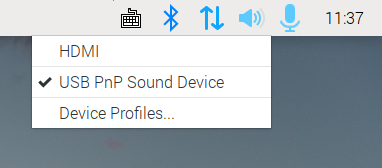
\includegraphics[width=0.8\textwidth]{select_sink.png}
    \caption{音声デバイスの選択と設定}
    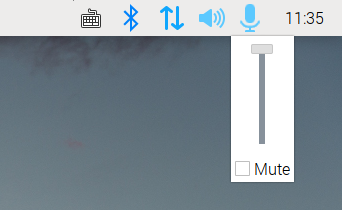
\includegraphics[width=0.8\textwidth]{microphone_volume.png}
    \caption{マイクの入力音量の調整}
  \end{figure}

\end{frame}

\begin{frame}
  \centering
  OpenJTalk
\end{frame}

\begin{frame}[fragile]
  \frametitle{文章を読み上げてもらう}
  
  \begin{lstlisting}[caption=openjtalk.hsp,label=openjtalk.hsp]
  #include "hsp3dish.as"
  #include "jtalk.as"

  redraw 0
  mes "発話開始"
  mes "「子どもIT未来塾」"
  redraw 1

  jtload "子どもIT未来塾", 0	<#blue#;音声ファイルを出力し、読み込む#>
  mmplay 0			<#blue#;音声ファイルを再生する#>
  stop
  \end{lstlisting}
\end{frame}

\begin{frame}
  \frametitle{問題を解こう}
  \begin{itemize}
    \item 教科書5ページ 問題6-3-1
    \begin{itemize}
      \item 2問(1問は宿題)
    \end{itemize}
    \item 教科書6ページ 問題6-3-2
    \begin{itemize}
      \item 3問(1問は宿題)
    \end{itemize}
    \item 教科書7ページ 問題6-3-3
    \begin{itemize}
      \item 2問(1問は宿題)
    \end{itemize}
    \item 教科書8ページ 問題6-3-4
    \begin{itemize}
      \item 2問(1問は宿題)
    \end{itemize}
  \end{itemize}
  
\end{frame}

\begin{frame}
  \centering
  Julius
\end{frame}

\begin{frame}
  \frametitle{Juliusを使ってみる(1)}
  \begin{itemize}
    \item run-linux-gmm.sh
    \item \<\<please speak\>\>がでるまで待つ
  \end{itemize}
  \centering
  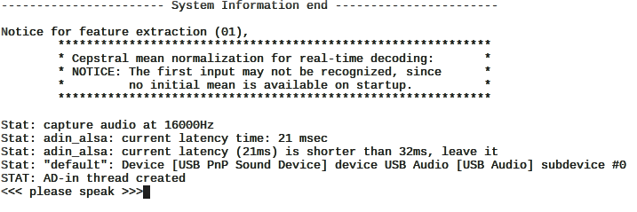
\includegraphics[width=0.8\textwidth]{chap06/text06-img009.png}
\end{frame}

\begin{frame}
  \frametitle{問題を解いてみよう}
  \begin{itemize}
    \item 教科書9ページ 問題6-4
    \begin{itemize}
      \item 1問
    \end{itemize}
    \item 教科書9ページ 問題6-4-1
    \begin{itemize}
      \item 1問
    \end{itemize}
  \end{itemize}
\end{frame}

\begin{frame}
  \frametitle{Juliusを使ってみる(2)}
  \begin{itemize}
    \item 果物の名前を話かけてみよう
    \begin{center}
      {\small りんご みかん ぶどう もも あけび あんず いちご いちじく かき スイカ すもも 	なし メロン}
    \end{center}
    \item 結果はどうかな?
    \item 話しかけた単語とターミナルに出てくる単語が同じか友達と話合ってみよう
  \end{itemize}
\end{frame}

\begin{frame}
  \frametitle{Juliusの限界}
  \centering 
  コンピュータは正しく言葉を認識してくれたかな?
  \note{画像を入れる}
\end{frame}
  
\end{frame}

\end {document}
